\documentclass[12pt]{article}
\usepackage[utf8]{inputenc}
\usepackage{subcaption}
\usepackage{graphicx}
\usepackage{float}
\usepackage{wrapfig}
\usepackage{authblk}
%\usepackage[
%top    = 0.25cm,
%bottom = 0.25cm,
%left   = 1.00cm,
%right  = 1.00cm]{geometry}
\usepackage[margin=1in]{geometry}

\title{ECS171 Final Report}
\author[1]{Patrick Chan}
\author[2]{Arnib Quazi}
\affil[1]{Email ID: plchan@ucdavis.edu}
\affil[2]{Email ID: arquazi@ucdavis.edu}
\date{June 4th, 2022}

\begin{document}

\maketitle

\newcommand{\CVItemListStart}{\begin{itemize}}
\newcommand{\CVItemListEnd}{\end{itemize}\vspace{-5pt}}
\newcommand{\TimelineStart}{\begin{itemize}}
\newcommand{\TimelineEnd}{\end{itemize}\vspace{-5pt}}

\section{Team Members}
Leader: Ninad Swadi\\
Group Members: Patrick Chan, Jai Malegaonkar, Arnib Quazi, Shlok Shah, Austin Rathkamp\\
 
\noindent [https://github.com/shlokshah7/ECS-171-project]
\section{Introduction}
Our team chose the project to be on Credit Card Approval. The data set we are using is, Credit Card Approval Prediction, A Credit Card Dataset for Machine Learning available on Kaggle.\\

\noindent According to the Consumer Financial Protection Bureau, approximately 45 million Americans do not have a credit score, preventing most from obtaining mortgages, car loans, and even personal loans. This problem stems from a lack of financial literacy among Americans and it’s costing millions of households thousands of dollars every year. The easiest way to build credit is through credit cards, where people can develop a credit history and improve their credit over time. Before applying for credit, people must meet a certain set of criteria like age of credit, income, cost of housing, etc. This data is then used by banks to determine credit worthiness and applicants are either approved or denied, with very little feedback given to applicants who were denied. We propose an ML model to help applicants gauge their creditworthiness before applying, helping them avoid an unnecessary credit score drop from a hard pull on their credit report. \\


\noindent Moreover FICO reports that while hard inquires does not impact already established good credit history. Our model is aimed towards those who are starting to build credit, or those who can't afford to record more hard inquires. This is because, again according to FICO, hard inquires for short credit history can be more damaging and those who have around 6 or more hard inquires are 8 times more likely to declare bankruptcy.\\

\noindent Our group performed unsupervised clustering techniques to determine any unique behavior that would allow us to better determine credit card approval, and we used supervised learning to create a model that predicts the approval of the users credit card via different features that does not need prior credit knowledge. How we determine this approval will be further discussed in Section 4 (Dataset Description)

\section{Literature Review}

\noindent In our dataset, we do not contain an out right credit score that we can use to determine credit card approval. The data does include the loan of certain IDs and their late day status. In order for us to justify using this as an indicator for credit card approval/risk we looked at J. Nalić and A. Švraka research paper on building a credit scoring model, in which they discover that late payments are the most important factor in their model for credit scoring. On top of that they're model which emphasized late payments was able to predict 95 percent of the credit risks and defaults, and the predictions were validated by the institution which wanted to employ their model.\\

\noindent Now that we have a justification for our target label, we moved on to researching other models built to predict credit card approval. In researching two different papers that created models, we see that linear regression is a great base model with a high accuracy but it is not necessarily the best. Zhao claims that SVM is the most accurate and Duan claims that a Neural Network is more accurate. However, neither accounts test both models.\\

\noindent However it is important to note that both papers use different data sets that already has a predefined approved variable, which could have a been based off a proprietary credit scoring model.\\

\noindent The research in the end concludes with a positive performance from their models with accuracy ranging from 87 percent on the high end and 66 percent on the lower end.\\

\noindent Our team's research will extend their research idea through analysis of individual attributes that affect customer purchases.\\

\section{Dataset Description}


\noindent The data set contains two separate CSV files. The first file named application record contains personal information on each applicant; such as income, education, occupation, etc. While the second file named credit record contains the age of a records loan account and if for any month they were late in paying their loan.\\

\noindent First it is important to note how credit record is structured. credit record is structured on a month to row basis. Meaning for every month a loan account is open, it will have that many rows in the file. So, while this file does use unique  IDs, each ID has multiple rows of loan data corresponding to that ID. Now of course this cause an indexing issue with the application credit, as that file only has one record per unique ID.\\

\noindent On the other hand, in the application record there are some duplicate inputs. Meaning while they have different unique IDs, the records have the exact same info. This could just be two separate applicant with different loan records or they might be the same applicant applying twice. In addition, their are some null values in application record.\\

\noindent The most important idea that needs to be addressed here is the need for feature engineering to create our target label or approval. We felt confident in creating this label from our literature review of  J. Nalić and A. Švraka, where they created a robust model that predicted credit risks which used late payments as the most important feature. However, we do coincide that using just late payments might not suffice in the most robust model.\\


\noindent Overall, their is necessary data prepossessing and exploratory analysis that must be done on our data set before any conventional models can be built\\

Link: https://www.kaggle.com/datasets/rikdifos/credit-card-approval-prediction\\

\section{Proposed Solution and Experimental Results}

\noindent For our data set, we decided to use supervised learning to train four different models to predict credit card approval: Logistic regression, XGBoost(decision tree), multi-layer perception, and Support Vector Machines. We also explored the use of unsupervised learning to find any underappreciated links between data points.\\

\subsection{Supervised Learning: Preprocessing}

\noindent Before we start building our model we had to address several issues as mentioned before. To begin we dropped the "FLAG MOBIL" label because every record in our data had the same value, 1. Next we merged the application data with the credit data on an inner merger with preserved the IDs between both sets. Doing so reduced our data set as not every ID that was in both files. Next we decided to change "DAYS BIRTH" to "YEARS OLD" and "DAYS EMPLOYED" to "YEARS EMPLOYED" so it is easier for users to input their data. Continuing the only NANs or NULLS were found in a a label called "OCCUPATION TYPE," instead of dropping these records we assumed that the applications simply did not fill in an occupation so we fill the values with "Not identified" value. Then we checked certain continuous variables through plotting them and found that "CNT CHILDREN," "AMT INCOME TOTAL," and "CNT FAM MEMBERS" had outlying values which caused these records to be dropped. Lastly for the application data we see that every record that is a Pensioner has an incorrect value for their "DAYS EMPLOYED" as logically if one is a pensioner then one does not work, so we set their "DAYS EMPLOYED" to zero and any "OCCUPATION TYPE" they have to "Unemployed"\\


\noindent Moving on we do a very simple creation of the target label based off of the late payment per month. In which a user has a score of 0 and points are deducted for how severe the late payment is and points are rewarded for payments on time. After a summing of the ID's total given account history, if the score is positive then the ID is approved while if the score is negative, then that ID is consider a risk and will not be approved. We also encoded the categorical labels using one hot encoding and standardized our data. Now with we search the processed data for any duplicates, which we classified as any IDs with the exact same info. We drop these duplicates here because if both their application data and loan statement data are an exact match, it is most likely they are duplicate applicants.\\

\noindent Lastly, We split our data into a 80/20 divide between our training and testing data set respectively. Here we can see a slight imbalance in our data, with 85 percent of our data points being approved and 15 percent not approved. To approve accuracy and to avoid a bias we use SMOTE to solve our imbalance.\\

\subsection{Supervised Learning: Model Creation}

\subsubsection{Logistic Regression}

\noindent The first model we trained was Logistic Regression, because it is a common algorithm to use for binary classification. Which for our instance would be approved or unapproved. For this model we applied hyper parameter tuning on the penalty used, inverse of regularization strength (C), Solver, and max iteration. While we did not test every possible value for C, we did find a best estimator with our values using a grid search cross validation. The following charts show the results of the trained model.\\

\noindent After training this model we have several indicators of its performance. The first one we checked was the Accuracy of the model, which was around 67 percent accurate or almost a coin toss. Besides that we have a decently high Area under the curve (AUC) score, which may be deceiving, however we can attribute this anomaly to the fact that our classifier achieves a good performance on the positive class (high AUC) at the cost of a high false negatives rate (or a low number of true negative). \\

\subsubsection{XGBoost}

\noindent The next model we trained was XGBoost or a popular distributed gradient-boosted decision tree. This is the only model which we did not get to hyper parameter train, but as we will see this model seems to our preform the others anyhow.
\begin{figure}[H]
    \centering
    \begin{minipage}[b]{0.5\textwidth}
        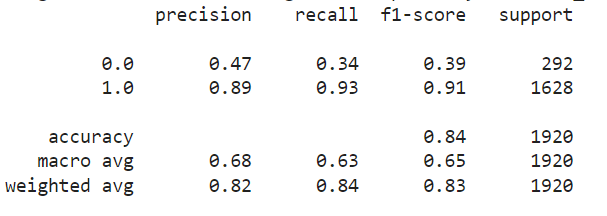
\includegraphics[scale = .45]{figures/XGBTable.png}
        \caption{XGBoost Classification Table}
    \end{minipage}
    \hfill
    \begin{minipage}[b]{0.4\textwidth}
        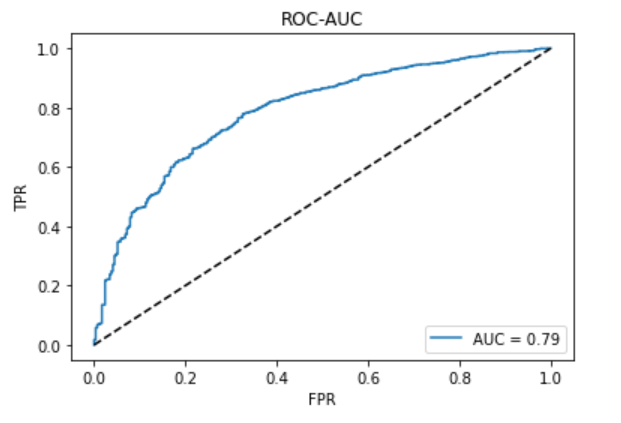
\includegraphics[scale = .30]{figures/XGB_roc.png}
        \caption{ROC and AUC graph}
    \end{minipage}
\end{figure}


\begin{wrapfigure}{r}{0.38\textwidth}
    \centering
    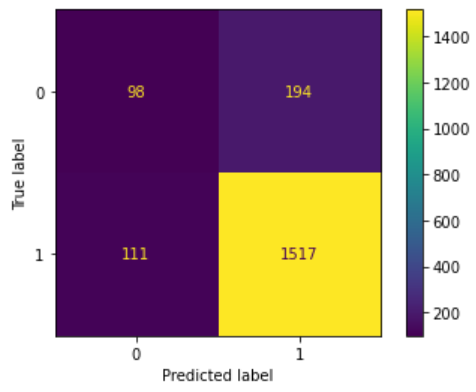
\includegraphics[scale = .30]{figures/XGBconf.png} 
    \caption{Confusion Matrix}
\end{wrapfigure}

\noindent This model achieved an overall 84 percent accuracy on the test set and a 95 percent on the original training set. The reason for this high accuracy is contributed how XGBoost minimises a L1 and L2 objective function that incorporates a function of convex loss and a  penalty term. In order to make the final prediction, the training continues iterative, inserting new trees that predict the residuals or errors of previous trees that are then combined with previous trees. Taking a further look at XGBoost's confusion matrix, there is a problem. When we calculate the false positive rate it amounts to around 66 percent. Which is unacceptable for our purposes, while this does have a great accuracy the fact that this model calculated 66 percent of unapproved clients as approved defeats our purpose.

\subsubsection{Feed Forward Neural Network}

\noindent Here we train a Feed Forward Neural Network, which was chosen due our prior literature review.
\begin{figure}[H]
    \centering
    \begin{minipage}[b]{0.525\textwidth}
        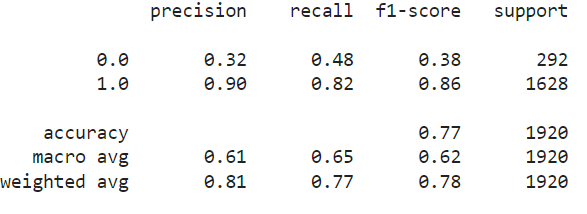
\includegraphics[scale = .45]{figures/FFNNTable.png}
        \caption{Feed Forward Neural Network Classification Table}
    \end{minipage}
    \hfill
    \begin{minipage}[b]{0.4\textwidth}
        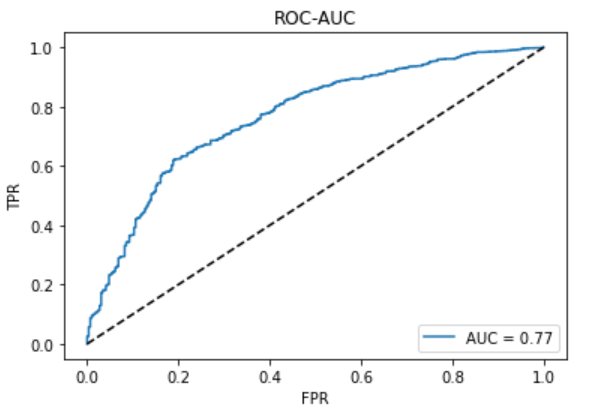
\includegraphics[scale = .30]{figures/FFNN_roc.png}
        \caption{ROC and AUC graph}
    \end{minipage}
\end{figure}


\begin{wrapfigure}{r}{0.38\textwidth}
    \centering
    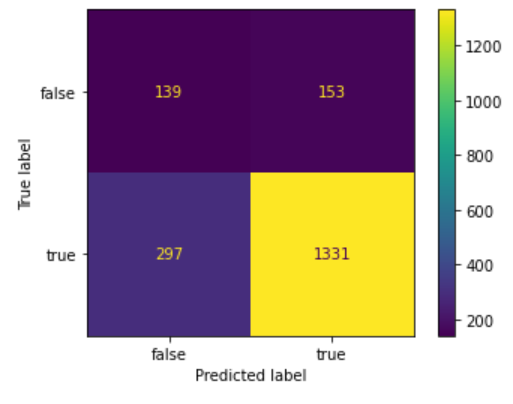
\includegraphics[scale = .30]{figures/FFNNconf.png} 
    \caption{Confusion Matrix}
\end{wrapfigure}

\noindent Here we hyper parameter tuned this model based on layer sizes, learning rate, and max iterations. Which is surface level training, for a better result we would continue to tune each layer's different parameters such as activation and size, as well as building the model with the Keras library. Overall, this model has an accuracy of 76 percent however it also suffers from a high False positive rate, which we can not justify. \\

\subsubsection{Support Vector Machine}

\noindent For support vector machine (SVM) we trained two different models, a SVM with a RBF kernel and one with a linear kernel. The RBF SVM suffers from the highest false positive rate, so instead we will focus on the linear SVM.\\

\begin{wrapfigure}{l}{0.38\textwidth}
    \centering
    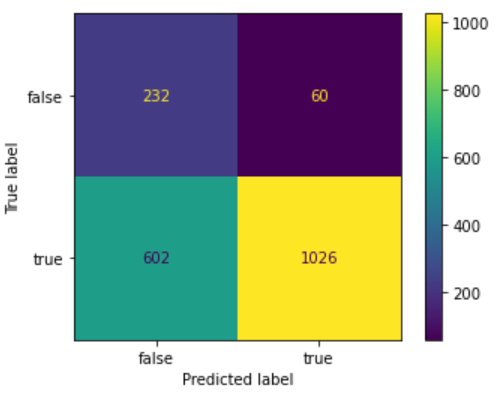
\includegraphics[scale = .30]{figures/LSVMconf.png} 
    \caption{Linear SVM Confusion Matrix}
\end{wrapfigure}

\noindent The Linear SVM has overall the worse accuracy for the models we trained, However we consider it to be the best model for our case. To justify this we will look at the confusion table. This model has the lowest false positive rate, meaning this model catches more not approved cases. It has approximately a 20 percent FPR which is still very high, but it is the best out of our models. \\ \\ \\ \\ \\

\subsection{Unsupervised Learning}

\noindent When we approached unsupervised learning, we took additional preprocessing steps to further reduce the amount of features we had. We first remapped the "STATUS" column (which originally had the values of \textbf{C, X, 0, 1, 2, 3, 4, and 5}) to just \textbf{0} and \textbf{1}. These original values represented how many days the particular individual was past due. The original values \textbf{C} (load was paid off), \textbf{X} (no loan taken), and \textbf{0} (1-29 days past due) were considered low risk and were thus given the value \textbf{1}. The other original values \textbf{1} (30-59 days past due), \textbf{2} (60-89 days past due), \textbf{3} (90-119 days past due), \textbf{4} (120-149 days past due) and \textbf{5} (Overdue or bad debts) were given the value of \textbf{0} as they were considered to be high risk. We then removed all duplicate values from the "ID" column. With preprocessing complete, we then begin our k-means clustering analysis.\\

\noindent We decided upon 6 potential features that we wanted to cluster one-on-one with "STATUS" column. These six features were "AMT\_INCOME\_TOTAL", "NAME\_INCOME\_TYPE", "NAME\_EDUCATION\_TYPE", 
"NAME\_EDUCATION\_TYPE", "DAYS\_EMPLOYED", and "MONTHS\_BALANCE". After clustering these features, we found that the only relevant feature seemed to be AMT\_INCOME\_TOTAL. \\

\begin{wrapfigure}{l}{0.55\textwidth}
    \centering
    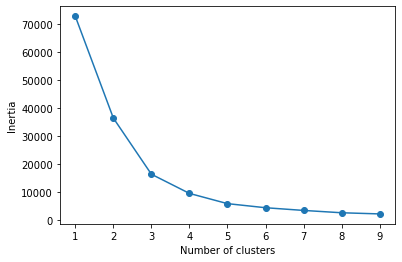
\includegraphics[scale = .6]{figures/output10.png} 
    \caption{Determining cluster count}
\end{wrapfigure}

\noindent As shown in Figure 8, we used the Elbow Method to determine that three clusters would work best for our analysis. After choosing three clusters, we then created the actual clustering between the total income and the approval status to get Figure 9. We concluded that the clustering found a link between income and approval odds and that \textbf{higher} incomes are \textbf{less risky} to lend to, while \textbf{lower} incomes are a considerably \textbf{higher risk} to lend to. \\

\begin{figure}[H]
    \centering
        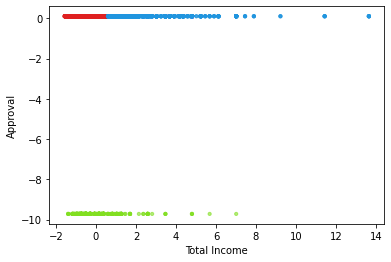
\includegraphics[scale = 1.0]{figures/output11.png}
        \caption{Clustering output from Total Income and Approval. Points near 0 are approvals while points near -10 are rejections}
\end{figure}

\section{Conclusion and Discussion}
\subsection{Supervised Learning}
Overall, out of the 5 models that were built we are left with 2 choices. The XGBoost with 84 percent accuracy or the Linear SVM with an 20 percent false positive rate. In the end we decided that false positive rate was a better metric for our models. This mainly coincides with our goal of building a model to help avoid damaging one's credit from unnecessary hard inquires. Also, it is important to note the imbalance in our testing data might also lead to a skewed accuracy in which misclassification of the false label has less of an impact than the misclassification of the positive label. Meaning because we only have 292 actual negatives or not approved out of a total of 1920 test samples, we can just predict all values as approved and still have an accuracy of about 86 percent.

\subsection{Model Synthesis}
After synthesizing all the data from the models, it is clear that two major factors present themselves as risk factors for late payments in our dataset: \textbf{Income} and \textbf{Property}. Those who had high income and owned property were highly unlikely to be late on payments, while those who had low income and did not own property were likely to be late on payments. This makes intuitive sense, as low income individuals can use credit cards as a form of short term supplemental income to buy necessities. The problem comes when the bill becomes due, as the extra money spent is not money these individuals have, so they require much more time to pay back their debts.

\subsection{Further Discussion}
When starting this project, we were under the belief that the data for this kind of analysis would be well established within dataset sharing communities like Kaggle. We could not have been more wrong. There exists very few datasets that have anywhere near the detail we would have liked to build a truly useful model for consumers to use. After conducting our analysis, we believe that our research is an incremental step forward in making these types of models more widespread and complete. We faced issues like heavy bias towards approvals, as opposed to rejections and a lack of data that aligns with FICO scoring methods (like total payment history or existing credit mix). There must be a push from larger lending firms like J.P. Morgan, American Express, Bank of America, etc. to make these types of datasets publicly available to analysts (like ourselves) who can create accurate and complete models for the general public to use. Done correctly, these types of models can even be used to bring in new groups of consumers that have historically stayed away from the credit system, presenting an exciting and new growth opportunity for lending firms. 
\\
\\
\\
\section{References}

https://www.myfico.com/credit-education/credit-reports/credit-checks-and-inquiries ( use proper format later)\\
\noindent Y. Zhao, "Credit Card Approval Predictions Using Logistic Regression, Linear SVM and Naïve Bayes Classifier," 2022 International Conference on Machine Learning and Knowledge Engineering (MLKE), 2022, pp. 207-211, doi: 10.1109/MLKE55170.2022.00047.\\

\noindent Y. Kang, R. Cui, J. Deng and N. Jia, "A novel credit scoring framework for auto loan using an imbalanced-learning-based reject inference," 2019 IEEE Conference on Computational Intelligence for Financial Engineering \& Economics (CIFEr), 2019, pp. 1-8, doi: 10.1109/CIFEr.2019.8759110.\\

\noindent L. Duan, "Performance Evaluation and Practical Use of Supervised Data Mining Algorithms for Credit Card Approval," 2020 International Conference on Computing and Data Science (CDS), 2020, pp. 251-254, doi: 10.1109/CDS49703.2020.00057.\\

\noindent J. Nalić and A. Švraka, "Using data mining approaches to build credit scoring model: Case study — Implementation of credit scoring model in microfinance institution," 2018 17th International Symposium INFOTEH-JAHORINA (INFOTEH), 2018, pp. 1-5, doi: 10.1109/INFOTEH.2018.8345543.

\end{document}